% Introduction

\pdfbookmark[1]{Quantitative revolutions}{Introduction}

\chapter{Quantitative revolution(s) in urban science}
\label{chap:quantitative_revolutions}

\begin{flushright}{\slshape    
And the first one now\\
Will later be last\\
For the times, they are a-changin'} \\ \medskip
--- Bob Dylan 
\end{flushright}


\bigskip


It is difficult to make a concise summary of what is known and not known about
urban systems. The vast amount of knowledge that has been gathered so far seems
very little in comparison to the bewildering complexity of the object being
studied~\cite{Batty:2008}. Every map, every satellite view, every statistic, every step
in cities elicits a question yet to be answered. What do we have to answer them?
A surprisingly small array of empirical tools and models. A surprisingly small
amount of solid, undisputed empirical facts.

Having said that, previous contributions are by no mean negligible. The body of
quantitative knowledge about cities has dramatically grown since the
quantitative revolution in Geography that took place after the $1950$s.
Recently, people have suggested that we may be witnessing the dawn of a second
quantitative revolution.\\

In the following Chapter, we will try to get some perspective on this claim, and
see to what extent it is justified. We will start with a (very) brief account of the
first quantitative revolution and the main themes around which it articulated
knowledge (a more comprehensive account can be found in~\cite{Sanders:2011}). We
will then critically review the factors traditionally invoked to justify the
spreading expression 'second quantitative revolution'.



\section{The first quantitative revolution}
\label{sec:the_first_quantitative_revolution}

Quantitative efforts in the study of human activities find their origin in Von
Th\"unen's model of agricultural land in $1826$, which suggests that the rent of land
should decay linearly with the distance to the city. More than a century later,
in $1933$, the German geographer Walter Christaller published his Central Place
Theory~\cite{Christaller:1933}, which aimed at explaining the size and location
of settlements in a system of cities. Needless to say, these early efforts are
theoretical in nature, and the empirical aspect -- studying things as they are
-- is left out. Surely due to the lack of available data.\\

The quantitative effort really starts to spread in the US in the
$1950$-$1960$~\cite{Berry:1993}. From the very beginning, the objective to make
geography a science is clearly stated. Starting with the introduction of Bunge's
seminal \emph{Theoretical Geography}, published in $1962$~\cite{Bunge:1962}.
According to the author, geographers can and should go beyond the mere
accumulation of facts, and try to discover the laws that rule the human and
physical phenomena occuring on the Earth's surface.   

Bunge proposed geometry as a tool to understand the observed pattern and
describe objectively the geographical space. The range of tools used quickly
expanded~\cite{Haggett:1966,Chorley:1968}, spanning stastistical
models~\cite{King:1969, Brunsdon:1998} -- whose importance is demonstrated by
the publication in $1969$ of Leslie King's \emph{Statistical Analysis in
geography}) -- and graph theory  -- as early as $1963$ with the publication of
Kansky's PhD thesis~\cite{Kansky:1963}. An early review of the use of graph
theory in geography can be found in Hagget and Chorley's
book~\cite{Haggett:1969}.\\

The research undertaken in the quantitative tradition can be -- tentatively --
divided in three different categories. First, the study of spatial
differentiation, aims at characterising the spatial patterns that result from
human activities. For instance, the study of population or employment densities
(see Part~\ref{part:polycentricity}), the local concentration of population
categories (see Part~\ref{part:segregation}), or the repartition of cities
inside a territory. 

Second, the study of spatial interactions. The progressive realisation that
distance is a critical factor to understand the arrangement of different spatial
phenomena led Tobler to state the First Law of Geography~\cite{Tobler:1970}. 

\begin{quote}
    Everything is related to everything else. But near things
    are more related than distant things.
\end{quote}

Linked to the study of spatial interactions is the (in)famous gravity model,
which states that the flow $F_{ij}$ between two locations $i$ and $j$ is given
by a function of the form

\begin{equation}
    F_{ij} = C\, P_i^\alpha\,P_j^\beta\, f(d_{ij})
\end{equation}

where $f$ is a decreasing function of distance. Although the analogy with
Newton's gravitation law was used by Reilly in $1931$ to find the retail market
boundaries between cities~\cite{Reilly:1931}, the above formulation in terms of
flows was formulated by Stewart in~\cite{Stewart:1948}. Note the competing
existence of Stouffer's theory of intervening
opportunities~\cite{Stouffer:1940}, according to which the flow between $i$ and
$j$ is proportional to the number of opportunities at $j$ and inversely
proportional to the number of opportunities between $i$ and $j$. It was
mathematically formulated later by Simini et al.~\cite{Simini:2012}.

Finally, the study of infrastructure. Starting with Kansky in
$1963$~\cite{Kansky:1963}, the study of the shape and growth of road networks,
railway networks and other infrastructure has witnessed a renewed interest
thanks to the study of spatial networks~\cite{Barthelemy:2011}.


\section{A second quantitative revolution?}
\label{sec:a_second_quantitative_revolution_}

People can be forgiven for believing that the present time bears any sort of
special character. But when we look closely enough, the change is perpetual, and
what is new now will be outdated tomorrow. During the past $3$ years, I have
at many times overheard the fact that we were currently witnessing a 'second
quantitative revolution' in the study of geographical systems. But is it really
the case? What differences with past tools or methods could justify such a
claim? In the following, we explore the three following hypotheses

\begin{itemize}
    \item The quantitative revolution is due to the availability of `new data';
    \item The quantitative revolution is due to the use of new methods coming
        from interdisciplinary studies;
    \item The new quantitative revolution is due to a technological convergence.      
\end{itemize}



\subsection{New methods}
\label{sub:new_methods}

The recent years have seen the application of new methods, mainly coming from
physics or computer science, to the study of cities. Either by geographers, or
outsiders who established well-established methods from another
field~\cite{Batty:1995}. These collaborations, or incursions, are however not
new. For instance, John Stewart, an american astrophysicists is famous for the first use of allometric
scaling in the study of cities~\cite{Stewart:1947}, or for his work 
on the gravitation model~\cite{Stewart:1948}. Another interesting example is
given by the collaboration in $1971$ between Waldo Tobler -- a geographer -- and
Leon Glass -- a chemist -- who plot the radial distribution function of Spanish
cities, a method that is traditionally used to study the property of
liquids~\cite{Glass:1971}.

So, the application of well-established methods from other fields to cities is
not new, and neither are the contributions made by outsiders. Yet, we can
identify two qualitative changes: the number, and nature of these contributions.
If some authors have continued to import directly methods and models from other
disciplines (for instance, the use of diffusion-limited aggregation models,
traditionally studied in physics, to explain the growth of
cities~\cite{Makse:1995}), this type of theoretical contribution is becoming
marginal. Contributions are more and more empirical; and if theoretical, are not
direct applications of another domain's theories. For
instance, Rozenfeld and co-authors used percolation on census tracts to define
cities~\cite{Rozenfeld:2008} in an original way. Masucci et al. use percolation
on the road network for the same purpose~\cite{Masucci:2015}, while Li et al.
use percolation to study the properties of congestion~\cite{Li:2015}. New
approaches to spatial network~\cite{Barthelemy:2011} have yielded new insights
into the structure and evolution of road, railway and subway networks~\cite{Strano:2012,
Barthelemy:2013,Louf:2013_emergence,Louf:2014_scaling,Louf:2014}.
Original out-of-equilibrium models that are inspired by the studied system allow
a better understanding: Simini's radiation model~\cite{Simini:2012,Simini:2013}
 -- which is nothing else that the mathematical transposition of Stouffer's
 intervening opportunities theory -- or our model to explain the polycentric
 transition of cities~\cite{Louf:2013_polycentric} are examples of such models.
 Not to forget the important literature on scaling
 relationships~\cite{Bettencourt:2007, Bettencourt:2013, Louf:2014_mobility,
 Arcaute:2014, Louf:2014_smog}, and other empirical analyses -- such as the
 study of residential segregation we present in Part~\cite{part:segregation}.
% Agent based model must be included somwehere here!

At the same time, the number of contributions to the field from authors who do
not have a geography (or economics, urbanism, etc. for that matter) affiliation
has been increasing over the pas years. After all, I am a theoretical physicist
by training, this thesis will be officially be registered as a theoretical
physics thesis. So, if the contributions of outsiders are not new, they are
changing in number and nature. To the point where we can wonder whether some of
these `outsiders' should still be considered as such.



\subsection{New data?}
\label{sub:new_data}

Besides the import of methods from other disciplines, it is often argued that
the influx of new data, thanks to the digitization of our lives, is a revolution
in itself. 

The most important new source of data come from the wide use of mobile phones
across the world~\cite{Gonzalez:2008,Fen-Chong:2012}. They consist, for each individual, of a
list of antenna location to which the individual was the closest at a given time
(either when he used the phone, or when he switched from an antenna to another).
Naively, one could think that mobile phone data are better than census-based
data: they give a \emph{continuous} information about the flow of individuals
within the city (and not only limited to commuting), they cover a larger part of
the population (which is critical in developing countries where censuses are not
widely used due to the costs involved, while mobile phones have a high
penetration rate), and are more spatially precise than released census data in
urban areas (see Figure~\ref{fig:IRIS_phone} for a comparison between the smallest
INSEE areal units, and mobile phone antennas in Paris). But one needs to be
careful. If mobile phone data are fine to monitor aggregate quantities (such as
origin-destination commuting matrices~\cite{Lenormand:2014}, or to map
population changes during the day~\cite{Louail:2014}, or year~\cite{Deville:2014}), one should be careful with the study of
individual trajectories (such as in the
seminal~\cite{Gonzalez:2008,Song:2010_modelling,Song:2010_limits}). Indeed, the
fact that positions are recorded every time a called is passed by the user,
events with a powerlaw inter-event time~\cite{Song:2010_modelling} and that are
probably correlated with locations, is likely to introduce an important biais in
the obtained trajectories. Not mentioning the spatial sampling introduced by the
fact that positions are attached to a finite number of antennas. Unfortunately,
there are no studies looking at the impact of these two samplings on the
properties of the observed trajectories. In the meantime, one should refrain
from using such data to study individual trajectories.

\begin{figure}
    \centering
    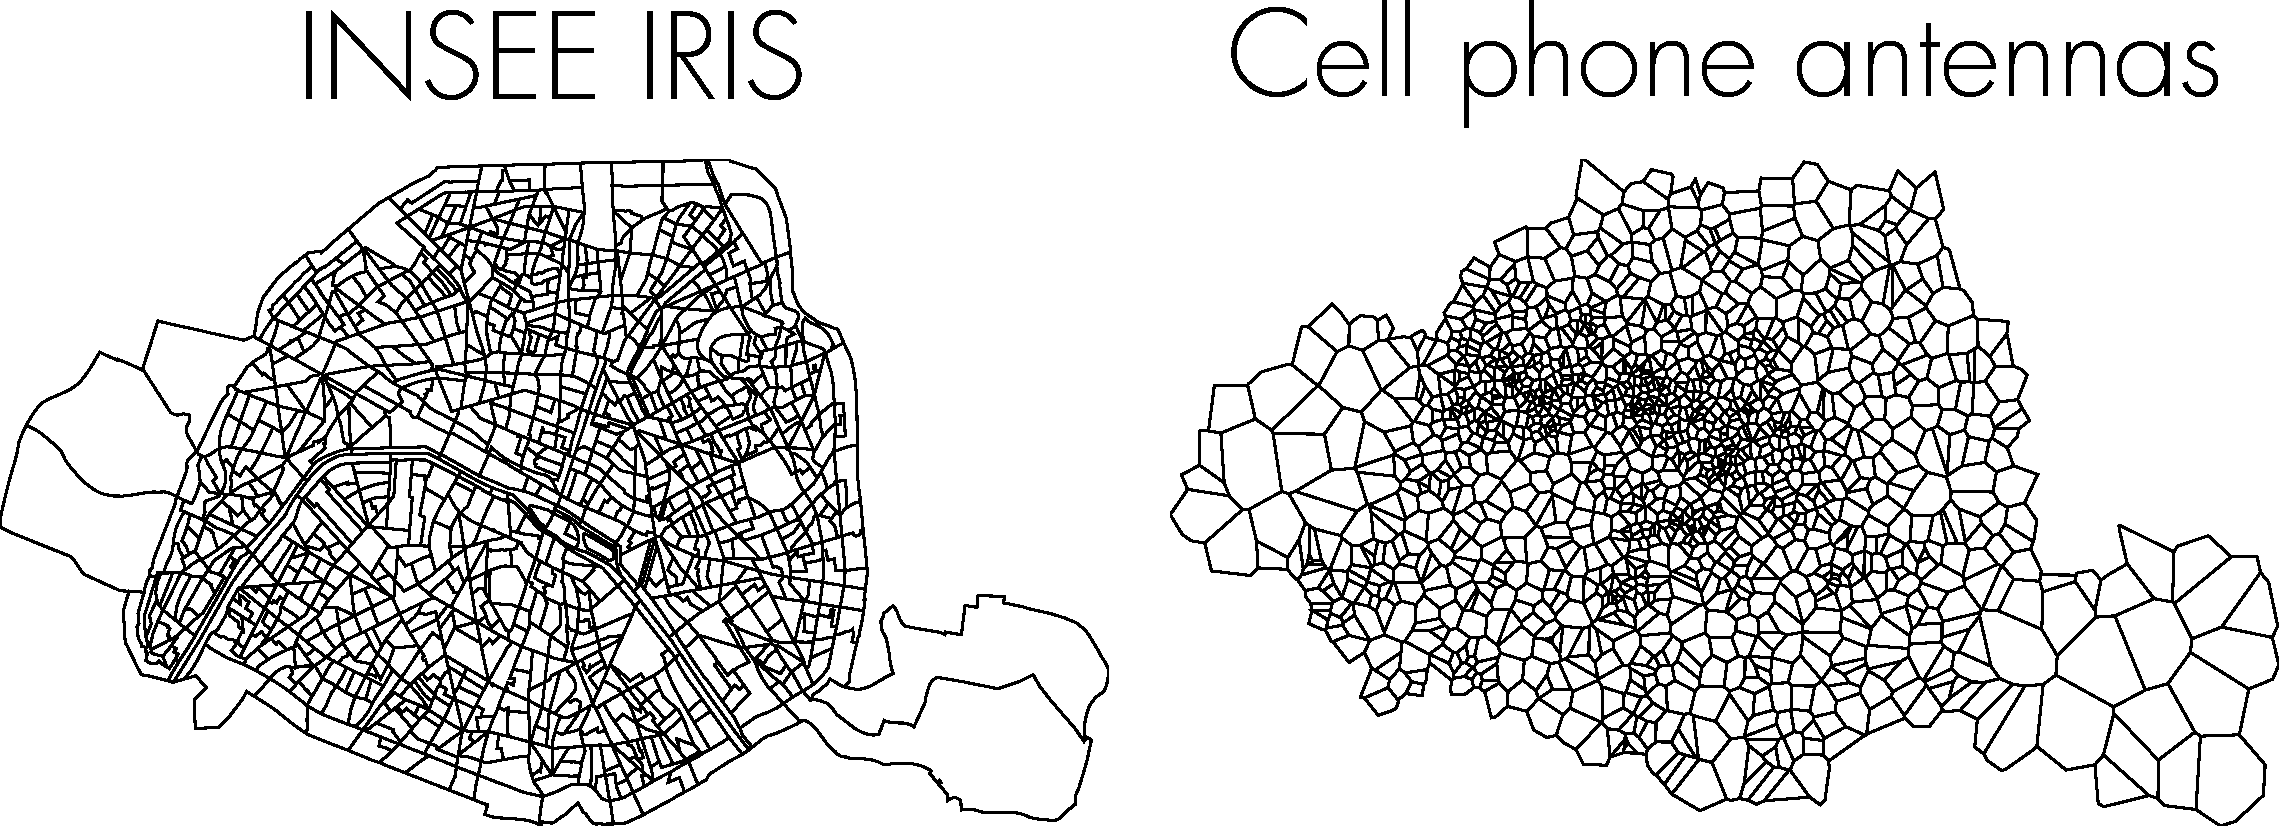
\includegraphics[width=\textwidth]{gfx/chapter-intro/IRIS_phone.pdf}
    \caption{(Left) IRIS zones in Paris, the smallest statistical units defined
    by the national statistics institute, INSEE. (Right) Voronoi tesselation
    built from the position of antennas of a popular french mobile phone carrier.
    There are $40\%$ more antennas than there are IRIS, and they tend to be more
    concentrated in zones of high daily activity (8th and 9th
    arrondissements).\label{fig:IRIS_phone}}
\end{figure}

Mobile phone data are not the only source of data. Because mobile phones carry
GPS chips that are used by certain applications, applications such as
FourSquare~\cite{Noulas:2012} or Twitter~\cite{Lenormand:2014_tweets}. Last, but
not least, Credit card companies have recently started to release datasets
regarding the spending of individuals~\cite{Lenormand:2015}.\\

So, new data (mainly mobile phone data) are now available and allow to give a
picture of the city that was before unavailable. The contribution of these new
data is particularly useful for the mobility of people besides commuting
pattern~\cite{Louail:2014}, or for developping country where there are little
census data available~\cite{Blondel:2012}. Are they so overlwhelmingly different
from previously available data to deserve the title of `revolution'? Nothing is
less certain: in this thesis, for instance, I have not used these `new data' at
all, and we are still waiting for important results that these data could teach
us and that we could not access with more traditional data. Only time will tell,
but the term `revolution' is certainly not warranted yet.



\subsection{A technological convergence}
\label{sub:a_technological_convergence} 

Interdisciplinary collaborations already existed, data were already there. So
what is the qualitative difference between the state of the field say $20$ years
ago, and the state of the field as it is now, if any? A factor that is often
overlooked is the recent technological leap in the treatment of information,
including spatial information. Thanks to the development of GIS software as well
as spatial databases and libraries, the treatment of geographical data has never
been simpler. Added to this are the emergence of powerful scripting languages, R
and Python, which allow to quickly implement complex data analysis workflow or
simulations, and reduce dramatically the time spent writing code. 

Internet is also progressively changing the way research is done. Census data
are more and more easily accessible available online. Open data repositories,
although far from perfect, are emerging. Online platforms such as
\url{www.github.com} allow to share and collaborate on code. All in all,
the access and processing of information is getting easier and easier.\\


Taken individually, the introduction of methods from other disciplines, the
increasing amount and specificity of available data and the technological
progresses in the treatment of information are probably not enough to justify
the term `revolution'. Taken together, however, they could mark the beginning of
a qualitative rupture in the way we understand cities.

It is too premature to conclude that the convergence of the aforementioned will
necessarily deeply change our understanding of cities. Only the future can tell
us whether new regularities, new laws are about to be discovered and more
phenomena to be understood. But where there is data, there is definitely hope.
Provided the correct methodology is used. In the following Chapter, we will
introduce the broad methodological prescriptions that were followed during this
thesis.
